
% \subsubsection{Computational Overhead}

% \begin{figure}
%   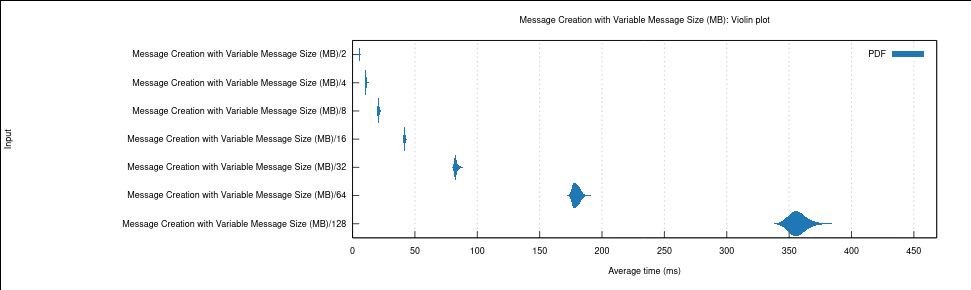
\includegraphics[width=\linewidth]{imgs/message_creation.png}
%   \label{fig:message_creation}
% \end{figure}
% In Figure 1 we see the time to run the first part of FACTS, that being $\send(u_1, u_2,m,tag_m)$. Looking at message construction we see that until the actual message content exceeds 64MB, creating and sending a message with the encrypted hash and identity takes sub 100ms, excluding the round trip network communication between the client and server. We see then that when a user wishes to forward a message, they will still call $\send(u_1, u_2,m,tag_m)$, but provide the server arbitrary data, and so if this data is less than 2MB, FACTS will add an overhead of only 5ms to this portion of the messaging system.

% \begin{figure}
%   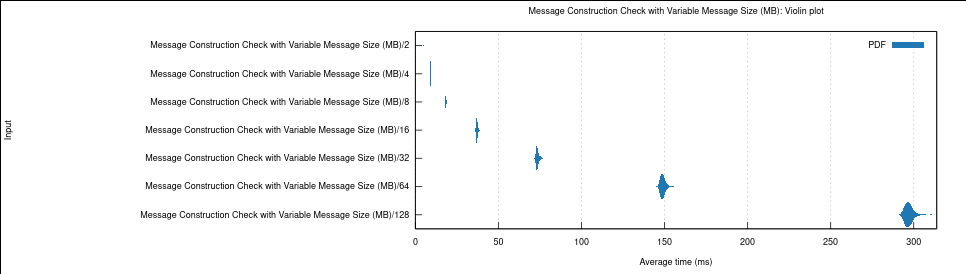
\includegraphics[width=\linewidth]{imgs/message_check.png}
%   \label{fig:message_check}
% \end{figure}
% Whenever a user receives a message, they must also check the construction of the message to ensure the encrypted identity and signature is valid, and has not been tampered with. We see in Figure 2 that for sub 64MB sized messages, FACTS adds only an overhead of at most 150ms.
% \begin{figure}
%   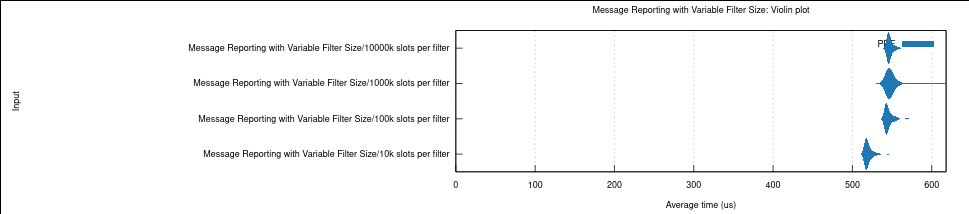
\includegraphics[width=\linewidth]{imgs/var_filter_size.png}
%   \label{fig:var_filter_size}
% \end{figure}

% \begin{figure}
%   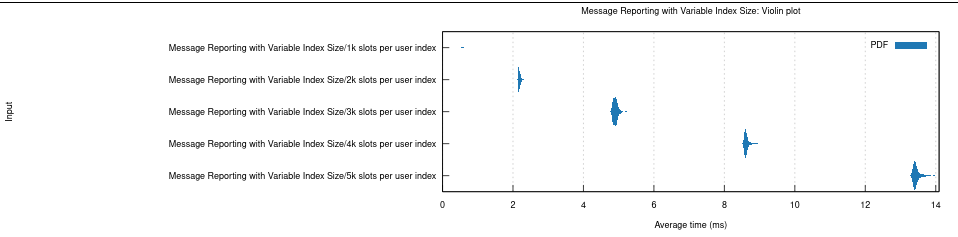
\includegraphics[width=\linewidth]{imgs/var_index_size.png}
%   \label{fig:var_index_size}
% \end{figure}
% Finally, we see in Figure 3 that  when a user wishes to actually report a message, there is almost no overhead, as with a fixed size of 1000 user bits, even when the Bloom filter reaches millions of slots, the process of reporting takes under a microsecond. In Figure 4 when we fix the size of the filter at 1 billion slots, we see even when a user's subset of bits is as large as 5000, the reporting process still takes under 15ms.

% \subsubsection{Network Overhead}
% 

